
\documentclass{book}

\author{Liliana Sanfilippo}
\usepackage[ngerman]{babel}

%% STANDARD 

\usepackage[english]{babel}
\usepackage[a4paper,top=2cm,bottom=2cm,left=1.5cm,right=1.5cm,marginparwidth=1.75cm]{geometry}

%% REFS / LINKS
\usepackage{amsmath}
\usepackage{hyperref} % Für klickbare Referenzen
\usepackage{cleveref} 
\hypersetup{
    colorlinks=true,
    linkcolor=blue,
    filecolor=magenta,      
    urlcolor=cyan,
    pdftitle={Overleaf Example},
    pdfpagemode=FullScreen,
    }


%% INDEX

\usepackage{makeidx} 
\makeindex

%% FIGURES

\usepackage{graphicx}

\usepackage{float}

\usepackage{caption}
\usepackage{subcaption}

%% COLUMNS

\usepackage{multicol}

%% BOXES 

\usepackage{tcolorbox}

\usepackage[dvipsnames]{xcolor}
\definecolor{myred}{HTML}{af5655}
\definecolor{mygreen}{HTML}{377771}
\definecolor{myblue}{HTML}{164254}
\definecolor{myyellow}{HTML}{D5BF86}
\definecolor{mygray}{HTML}{8AA1B1}

\usepackage{amsthm}
\newtheoremstyle{mytheoremstyle} % name
    {\topsep}                    % Space above
    {\topsep}                    % Space below
    {}                   % Body font
    {}                           % Indent amount
    {\bfseries}                   % Theorem head font
    {}                          % Punctuation after theorem head
    {1.5em}                       % Space after theorem head
    {\thmname{#1}\thmnumber{ #2}\thmnote{ #3}}  % Theorem head spec (can be left empty, meaning ‘normal’)
\theoremstyle{mytheoremstyle}

\newtheorem{bsp}{Beispiel}[section]

%\newtheorem{formel}[defi]{Definition}
%\newtheorem{gese}{Gesetz}[section]

%% DEFINITION

\newtheorem{defi}{Definition}[section]

\newcommand{\defin}[1]{
\begin{lavenderbox}{\textbf{\gls*{#1}}}
\noindent
\begin{defi}
    \glsdesc*{#1}
\end{defi}
\end{lavenderbox}
}
\usepackage[automake]{glossaries}

\newglossary[vlg]{defi}{vls}{vlo}{Definitonen}

\newglossary[flg]{fragen}{fls}{fls}{Fragen}

\newglossary[rlg]{regeln}{rls}{rls}{Regeln}

\newglossary[slg]{satz}{sls}{sls}{Sätze}


\newglossary*{dinge}{Was ist was?}
\glsaddkey
{formB}
{}
{\glsentryB}
{\GlsentryB}
{\glsB}
{\GlsB}
{\GLSB}
\glsaddkey
{formF}
{}
{\glsentryF}
{\GlsentryF}
{\glsF}
{\GlsF}
{\GLSF}


\newglossary[slg]{symbolslist}{syi}{syg}{Symbole und Begriffe} % create add. symbolslist

\makeglossaries

%\glsaddkey{unit}{\glsentrytext{\glslabel}}{\glsentryunit}{\GLsentryunit}{\glsunit}{\Glsunit}{\GLSunit}
\glsaddkey{verb}{\glsentrytext{\glslabel}}{\glsentryverb}{\GLsentryverb}{\glsverb}{\Glsverb}{\GLSverb}



% masculine nominative
\glsaddkey
{nominative}% key
{}% default value
{\glsentrymnominative}% no link cs
{\Glsentrymnominative}% no link ucfirst cs
{\glsmnom}% link cs
{\Glsmnom}% link ucfirst cs
{\GLSmnom}% link all caps cs

% masculine accusative
\glsaddkey
{accusative}% key
{}% default value
{\glsentrymaccusative}% no link cs
{\Glsentrymaccusative}% no link ucfirst cs
{\glsmacc}% link cs
{\Glsmacc}% link ucfirst cs
{\GLSmacc}% link all caps cs

% masculine genitive
\glsaddkey
{genitive}% key
{}% default value
{\glsentrymgenitive}% no link cs
{\Glsentrymgenitive}% no link ucfirst cs
{\glsmgen}% link cs
{\Glsmgen}% link ucfirst cs
{\GLSmgen}% link all caps cs

% masculine dative
\glsaddkey
{dative}% key
{}% default value
{\glsentrymdative}% no link cs
{\Glsentrymdative}% no link ucfirst cs
{\glsmdat}% link cs
{\Glsmdat}% link ucfirst cs
{\GLSmdat}% link all caps cs



% masculine nominative
\glsaddkey
{nominativepl}% key
{}% default value
{\glsentrymnominative}% no link cs
{\Glsentrymnominative}% no link ucfirst cs
{\glsmnom}% link cs
{\Glsmnom}% link ucfirst cs
{\GLSmnom}% link all caps cs

% masculine accusative
\glsaddkey
{accusativepl}% key
{}% default value
{\glsentrymaccusative}% no link cs
{\Glsentrymaccusative}% no link ucfirst cs
{\glsmacc}% link cs
{\Glsmacc}% link ucfirst cs
{\GLSmacc}% link all caps cs

% masculine genitive
\glsaddkey
{genitivepl}% key
{}% default value
{\glsentrymgenitive}% no link cs
{\Glsentrymgenitive}% no link ucfirst cs
{\glsmgen}% link cs
{\Glsmgen}% link ucfirst cs
{\GLSmgen}% link all caps cs

% masculine dative
\glsaddkey
{dativepl}% key
{}% default value
{\glsentrymdative}% no link cs
{\Glsentrymdative}% no link ucfirst cs
{\glsmdat}% link cs
{\Glsmdat}% link ucfirst cs
{\GLSmdat}% link all caps cs





\loadglsentries{../bio_gloss}
\loadglsentries{glossary/definitionen}
\loadglsentries{glossary/fragen}
\newtcolorbox{lavenderbox}{colback=white,
colframe=Lavender}
\newtcolorbox{cyanbox}{colback=white,
colframe=Cyan}
\newtcolorbox{orchidbox}{colback=white,
    colframe=Orchid}

\newcommand{\txc}[1]{
\textcolor{red}{#1}
}



%% BIBTEX

\usepackage{biblatex}
\addbibresource{bib.bib}

\title{Eukaryotengenetik \\ \small{by Frau Gentz} \\ \textit{\footnotesize{Summer semester 2026} } }

\newcommand\reporttitle{Vorlesung Eukaryotengenetik}
\newcommand\reportsubtitle{Sommersemester 2026}
\newcommand\profs{Vorlesung von Prof. Weisshaar}
\newcommand\reportsubsubtitle{Vorlesungsnotizen und Aufarbeitung}
\newcommand\reportauthors{
    \textbf{Liliana Sanfilippo}
}

\begin{document}

    \frontmatter
    %! Author = lili
%! Date = 5/31/26

\makeatletter
\newcommand{\gettikzxy}[3]{%
    \tikz@scan@one@point\pgfutil@firstofone#1\relax
    \edef#2{\the\pgf@x}%
    \edef#3{\the\pgf@y}%
}
\makeatother

\begin{titlepage}

    \centering

    \begin{tikzpicture}

        \node[inner sep=0pt] (logo) at (0,0)
            {
\includegraphics[width=.25\textwidth]{../preamble/notes-notepad-svgrepo-com}};

        \node[text width = 0.5\textwidth, right = of logo](title){\sffamily\huge\reporttitle};

        \node[text width = 0.5\textwidth, yshift = 0.75cm, below = of title](subtitle){\sffamily\Large \reportsubtitle};

        \gettikzxy{(subtitle.south)}{\sffamily\subtitlex}{\subtitley}
        \gettikzxy{(title.north)}{\titlex}{\titley}
        \draw[line width=1mm, kapitelf]($(logo.east)!0.5!(title.west)$) +(0,\subtitley) -- +(0,\titley);

    \end{tikzpicture}
    \vspace{5cm}

    \sffamily\large\reportsubsubtitle

    \sffamily\large\reportauthors


    \vspace{5cm}
    %\sffamily \textcolor{black!80}{\placeanddate} \\


    %\tikz[remember picture,overlay]\node[anchor=south,inner sep=0pt] at (current page.south)
    %{\includegraphics[width=\paperwidth]{Figures/0. General/footer.pdf}};

    \mbox{}



\end{titlepage}










    \tableofcontents

    \mainmatter
    \chapter*{Infos}
    Empfohlene Literatur:

    \begin{itemize}
        \item Lewin’s GENES XII, Jones \& Bartlett publishers 2017 (ISBN 978-1-284-10449-3)
        Jocelyn E. Krebs, Elliott S. Goldstein, Stephen T. Kilpatrick
        \item Lewin’s GENES XI, Jones \& Bartlett publishers 2013 (ISBN 978-1-4496-5985-1)
        Jocelyn E. Krebs, Elliott S. Goldstein, Stephen T. Kilpatrick
        \item Molekularbiologie, 6.\ Aufl.\ Pearson 2011 (ISBN 978-3-86894-029-9)
        Watson / Baker, Bell, Gann, Levine, Losick
        \item Genetik, Thieme Verlag 2008 (2.\ Auflage) (ISBN 3-13-128771-3)
        Wilfried Janning, Elisabeth Knust
    \end{itemize}

    \chapter{Themenübersicht, Einführung, Wiederholung}
    \section{"Milestones" der Molekularbiologie/Genetik}
\txc{Füge ich nach, falls tatsächlich relevant.}

\section{Das zentrale Dogma der Molekularbiologie}

\begin{center}
    ``The central dogma states that information in nucleic acid can be perpetuated or transferred, but the transfer of
    information into protein is irreversible''
\end{center}

\begin{center}
    ``DNA macht RNA macht Protein''
\end{center}

\defin{dogma}

\begin{figure}[H]
    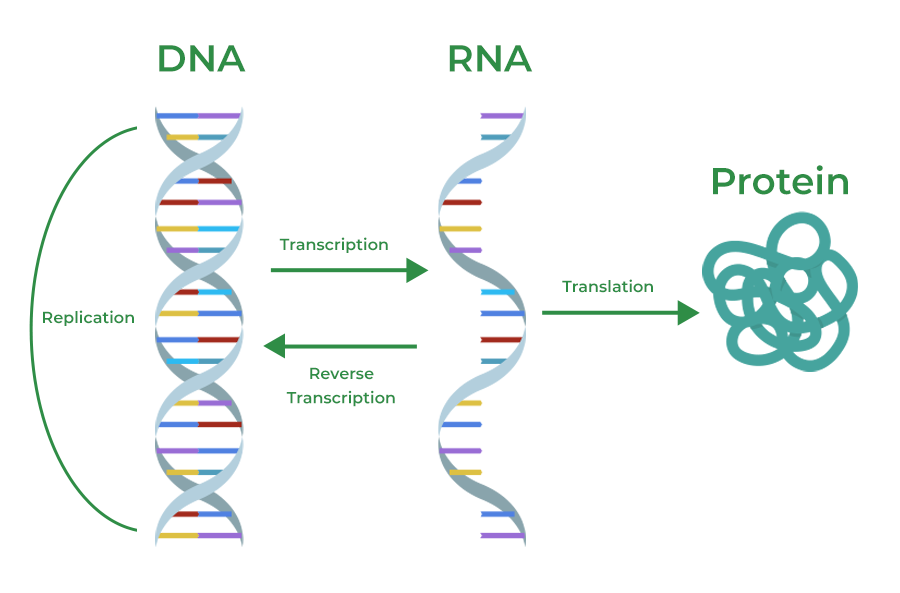
\includegraphics[width=\textwidth]{images/dogma}
    \caption{Code Sonne von \url{https://www.geeksforgeeks.org/biology/central-dogma-steps-guide/}}
\end{figure}


% TODO F 33- 35

\section{Der gentische Code}

\begin{figure}[H]
    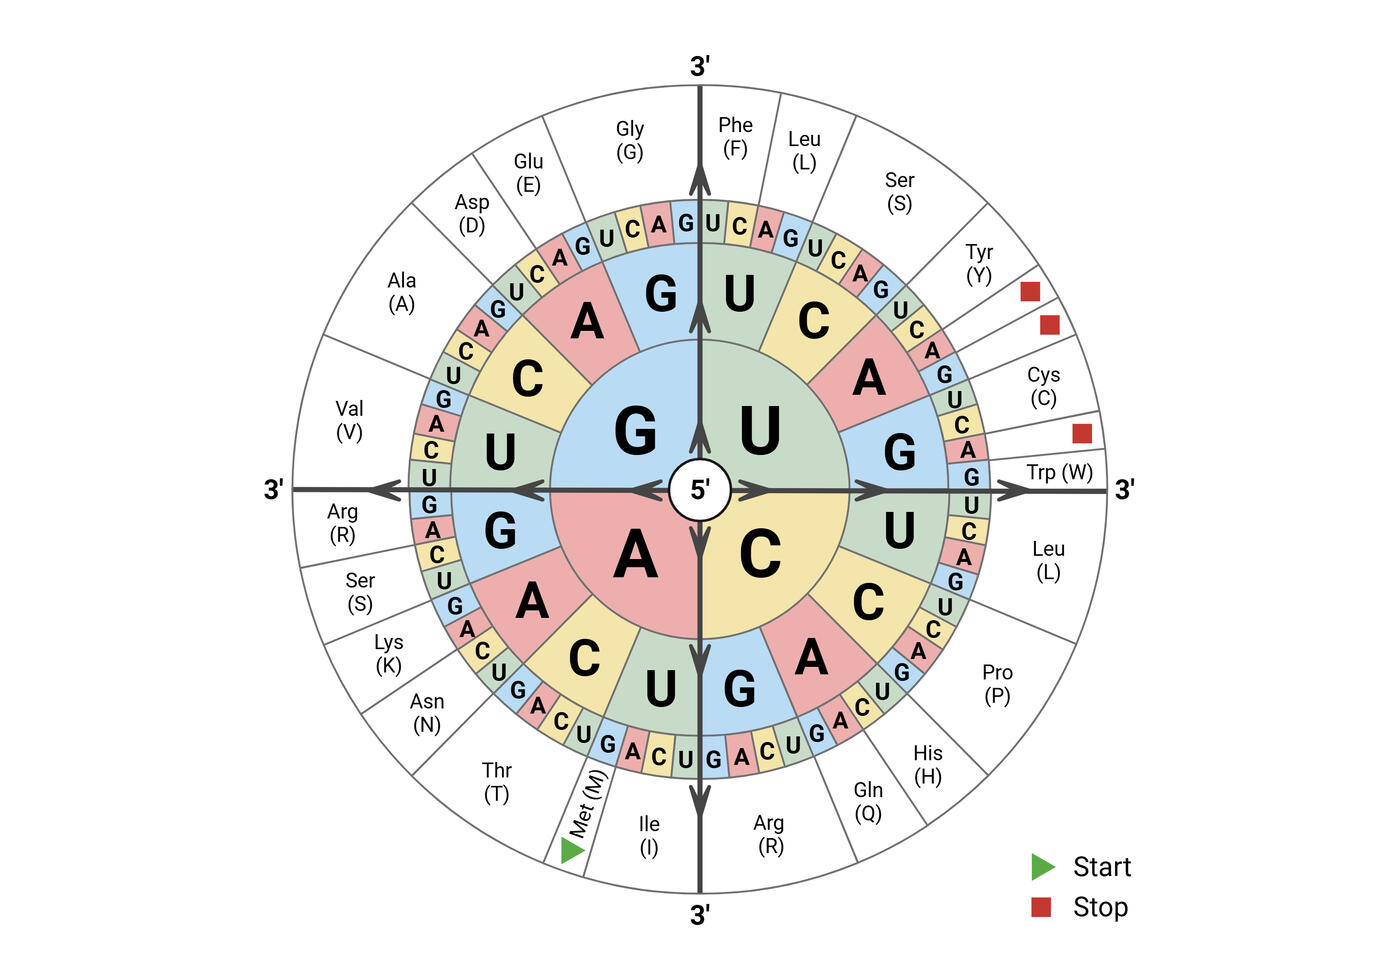
\includegraphics[width=\textwidth]{images/code_sonne}
    \caption{Code Sonne von \url{https://www.openscience.or.at/de/wissen/genetik-und-zellbiologie/2013-03-10-der-genetische-code/}}
\end{figure}

\section{Eukaryotisches "Muster-Gen"}

\begin{figure}[H]
    % TODO Bild
    \caption{Pol II}
\end{figure}


\section{Exons und Introns}

% TODO BILD

Gene mit drei Exons finden Sie in Lehrbüchern immer wieder, diese sind aber real eher selten.
Das ATG muss nicht im ersten Exon sein (und das ATG bestimmt KEINESFALLS den Anfang eines Exons)


    \chapter{Pro- vs Eukaryoten; Gene und Genome}
    %! Author = lili
%! Date = 5/7/26

\begin{table}[H]
    \centering
    \begin{tabular}{p{6cm} p{6cm}}
        \textbf{Prokaryoten} & \textbf{Eukaryoten} \\
        \hline

        kernlose Zellen &
        kernhaltige Zellen \\

        evolutionär älter &
        Endosymbionten-Theorie (Organellen, ausgeprägte Kompartimentierung) \\

        Genorganisation in Operons (polycistronische mRNA) &
        Genomorganisation in Genen (i.d.R.\ monocistronische mRNA) \\

        Genexpression: Promotor/Operator &
        komplexe Genexpression (RNA Pol-II) \\

        wenig bis keine Introns &
        Gene mit Introns als Regel \\

        Translation am nascenten Transkript &
        Polyadenylierung, Cap-Struktur \\

        „einfache“ Zellteilung &
        Trennung von Transkription und Translation in Kern und Cytoplasma \\

        &
        Mitose, Meiose \\
    \end{tabular}
    \caption{Prokaryoten vs. Eukaryoten}\label{tab:prokaryoten-vs-eukaryoten}
\end{table}

\section{Gene}
Gene liegen auf Chromosomen und sind linear angeordnet.
\paragraph{Was ist ein Gen?}
Naive Annahme:

\begin{center}
    Ein Gen codiert für ein Protein.
\end{center}
Das ist jedoch nicht ganz ausreichend.
Differenzierter könnte man sagen:
\begin{center}
    Ein Gen umfasst den gesamten Bereich auf der DNA, der zur Erstellung
    einer (m)RNA notwendig ist, einschliesslich der regulatorischen Regionen.
\end{center}
Das passt ``so halb'' für Prokaryoten, bei denen Gene oft hinter Operons liegen und daher durch das Operon an einem
Stück transkribiert wird.
Es entsteht eine mRNA, aber diese kann immer noch für mehrere Proteine kodieren.

Für Eukaryoten passt es nicht.
Denn es bezieht nicht ein, dass bei Eukaryoten Gene ``ineinander'' liegen können.
Ein DNA-Bereich kann bei einem Gen ein Intron sein und bei einem anderen Gen ein kodierender Bereich.
Aufgrund der Leseraster kann die DNA-Sequenz auf verschiedene Arten gelesen werden.
Außderdem können Exons beim Spleißen verschieden zusammen gefügt werden.

\frage{wasistgen}

\begin{bem}
    Bei Bakterien und Archaeen sind
    Genzahl und Genomgröße proportional.
    Bei Eukaryoten:
    Keine Korrelation der Genzahl mit Genomgröße oder Komplexität des Organismus.
\end{bem}

Wie findet man sich in so viel DNA bzw. Genen zurecht?

\begin{itemize}
    \item Restriktionskartierung (Beispiel: DNA Tumorviren, etwa Adenovirus-2)
    \item BAC-Contigs (Beispiel: Physikalische Karte von Arabidopsis thaliana)
\end{itemize}

% TODO
\frage{wiekarte}

    \chapter{Eukaryotische Genome, DNA Replikation}
    %! Author = lili
%! Date = 5/7/26

\section{Introns}
\begin{bsp}
    Vorkommen in verschiedenen Aktin Genen % TODO F 7
\end{bsp}

\paragraph{Eine Frage der Genomevolution} ist:
Haben sich Gene zunächst mit Introns entwickelt,
oder enthielten frühe Gene keine Introns?

Dazu gibt es verschiedene Modelle und Hypothesen:
\model{introns-late}
\hypothese{introns-first}
\hypothese{exon-shuffling}

\frage{wieintrons}


    \chapter{mRNA-Struktur, Initiation der Transkription}
    %! Author = lili
%! Date = 5/24/26
% 63 Folien
% TODO Unklar F 47, F 50

\untit{F. 1--8 Intro u. Wdh.}

\section{Einordnung der Transkription}
% TODO F 9-11

\section{RNA-Klassen in Eukaryoten}
% TODO F 13

\section{RNA Polymerasen}
% TODO F 14 - 20
% TODO F 31 - 32

\section{Aufbau der eukaryotischen mRNA}
% TODO F 22 - 30

\section{Promotoren - Start der Transkription}
% TODO F 33 - 41
% TODO F 48 - 49, 51 - 52, 55 - 57

\section{Transkriptionsfaktoren}
% TODO F 53 - 54, 58 - 59

\section{Elongation}
% TODO F 60 - 62

\section{Termination der Transkription}
% TODO F 42 - 46

\section{Genetische Regulation}
% TODO F 21



    \chapter{Spleißen (splicing), RNA Editierung}
    %! Author = lili
%! Date = 5/24/26
\untit{Kapitel 19+ in Lewin's Genes II}
% TODO Unklar F 20 - 22, 42

\untit{F. 1--10 Intro u. Wdh.}
% TODO schauen, dass das an anderer Stelle tatsächlich vorkommt

\section{Kontrollebenen der Regulation}
% TODO F 11

\section{Spleißen}
% TODO F 12 - 32

\subsection{Nucleäres Spleißen}

\begin{figure}[H]
    % TODO F 18 - 19
    \caption{Vergleich: Prozessierung der rRNA}
\end{figure}


\subsection{splice sites}

\subsection{Lariat-Struktur}

\subsection{Ablauf}

\section{Das Spleißosom}
% TODO F 33 - 37

\section{Intron- und Exon-Erkennung}
% TODO F 38 - 40

\section{Alternatives Spleißen}
% TODO F 43 - 48

\section{Spleißen und Krankheiten}
% TODO F 41

\section{RNA - Editierung}
% TODO F 50 - 56

    \chapter{Transposons, T-DNA, Transformation}

    \chapter{Nukleosomen, Chromatinstruktur, PTGS und miRNA}

    \chapter{Protein-Lokalisation und -Transport in der Zelle}

    \chapter{Immungenetik, Antikörper-Gene, "VDJ-joining”}

    \chapter{Zellzyklus, Kontrolle der Zellteilung}

    \chapter{Humangenom, Erbkrankheiten, "Onkogene”}

    \chapter{Genetik des Modellsystems A. thaliana}

    %! Author = lili
%! Date = 5/6/26

\section{Nukleosomen und Histonvarianten}\label{sec:nukleosomen-und-histonvarianten}

% begriffe für Karteikarten: Histonoktamer,
% Ich sollte laut reden, nicht ablesen und nicht gestelzt Begriffe wie Histonoktamer statt Histon benutzen
% Er fragt gerne, was das mit der Bioinformatik zu tun hat

%\paragraph{Sollten wir die Histonvarianten für die Klausur kennen?}

\paragraph{F 7: Welche Variante macht was oder macht jede Variante alles davon?}  Nicht jede macht alles, kann man
auf anderer Folie sehen, war da nur nicht mit drauf was was ist.

\paragraph{F 8: was meinst du mit Histone "markieren" verschiedene Transkriptionszustände?} Man könnte es einfach
daran erkennen.
Theoretisch, aber auch man könnte auch Antikörper produzieren lassen, die an bestimmte
Modifikationen binden und sie so praktisch markieren.

\paragraph{F 8: Ich habe nicht verstanden was ein +1 Nukleosom ist. Ist das da abgebildet?} Ja, ganz klein.
Das ist einfach das, was an der +1 Stelle ist und das kann eines von 4 möglichen Nukleosomen sein.

%\paragraph{F 11: Kommt H2A.Z bei allen Brustkrebsvarianten vor oder nur bei bestimmten?}

Weitere:
\paragraph{Kann man H2A.Z in macroH2A umwandeln?} Nicht beantwortet, Frage passt nicht zu Funktionalität.

\section{Genetic variation across and within individuals.}\label{sec:genetic-variation-across-and-within-individuals.}
% nicht mit dem Rücken zum Publikum, nicht einfach alles vorlesen aus Abbildungen...vor allem nicht einfach alles auf
% Deutsch vorlesen, was da auf eng steht, tabellen mit text sind keine guten Abbildungen, folienzahlen!
% Wtf mal nicht Leute unterbrechen, die Fragen stellen, rude
% Typen von Folgen (loss of function, etc.)

% Gut war Fazit & Rückbeziehung und Diskussionsfolie

% begriffe: extrinsische und intrinsische Motivationsstellen, somat. vs. Keimbahnmutationen (Art), typen mutationen:
% Substitutionen (SNV), Insert/Deletion < 50bp (Indels), ... weitere

% Art vs Typ bei Mutationen

Frage: Was ist SNV vs SNP

% große Abbildungen lieber auf Folien aufteilen statt zoomen

% Auswirkungen von Keimbahn- bzw. somat. Mutationen auf den Organismus

% man kann nicht immer sagen, ob insertion oder deletion vorliegt -  warum?


% In der Vorlesung haben wir gelernt, das unter bestimmtem Mutagenese-Einwirkungen (Bspw. UV vs andere) vorzugsweise
% in bestimmte Basen übergehen? Irgendwie sowas meinte Sagasser

\section{Plasmodesmata and intercellular molecular traffic control}\label{sec:plasmodesmata-and-intercellular-molecular-traffic-control}
Nüscht

\section{On the genetic basis of tail-loss evolution in humans and apes.}\label{sec:on-the-genetic-basis-of-tail-loss-evolution-in-humans-and-apes.}
Nüscht
% Vorwärtsgenetik vs. Rückwärtsgenetik



% Dritter Tag
\section{The emerging view on the origin and early evolution of eukaryotic cells}\label{sec:begin-of-eukaryotic-cells-oder-so}
% Zweidomänen-Modell
Nachschlagen: Protein-Struktur vergleichen statt Sequenz, um echte Neuheiten von unerkannten Homologen zu trennen
% "ich habe was ganz grundlegendes vergessen und frage einfach mal" come on

\section{Structure and Function of the 26S Proteasome}\label{sec:structure-and-function-of-the-26s-proteasome.}
% Proteasom, ubiquitin in defis packen, auch das Wort sterisch
RPN11 ist essenziell, hat man über Mutantenanalyse herausgefunden


    \backmatter
    \pagenumbering{roman}


    \chapter{Backmatter}\label{ch:backmatter}

    \addcontentsline{toc}{section}{Figures}
    \listoffigures

    \addcontentsline{toc}{section}{Index}
    \printindex

    \addcontentsline{toc}{section}{Definitions}
    \printglossary[type=defi, title=Definitions]

    \addcontentsline{toc}{section}{References}
    \printbibliography

\end{document}
